\InputIfFileExists{../data/global.tex}\relax\relax

\iffull
\title{Von Erben, Scherben und dem Schnittstelle-werden}
\subtitle{The final Tut}
\date{KW 29}
\addbibresource{references.bib}
\fi
\SetTutoriumNumber{11}

\iffull\begin{document}
\titleframe

\TopicOverview{5}
\fi

\iffull{\SummaryFrame
\begin{frame}[c]{Kurzwiederholung}
\vspace*{1em}
\begin{center}
    \onslide<2->{Diesmal am Ende, als Zusammenfassung!}
\end{center}
\end{frame}
}\fi

% \SetNextSectionText[.6\linewidth]{TODO}
\section{Präsenzaufgabe}
{
\begin{frame}[fragile,c]{Präsenzaufgabe}
\begin{aufgabe}{Dir streichen wir das Erbe!}
\only<2-3|handout:0>{Gegeben sei die folgende abstrakte Klasse \T{RegularPolygon}, welche ein Polygon mit gleichen Seitenlängen bzw. Innenwinkeln repräsentieren soll:}\only<4->{\vspace*{-1.75em}}%
\lstfs{9}%
\begin{minted}{java}
/*\CodeFileMarkerAttach<3->{RegularPolygon.java}*/
/*\onslide<3->*/public abstract class RegularPolygon {
/*\onslide<3->*/    protected final int numSides;
/*\onslide<3->*/    protected final double sideLength;
/*\onslide<3->*/    public RegularPolygon(int numSides, double sideLength) {
/*\onslide<3->*/        this.numSides = numSides;
/*\onslide<3->*/        this.sideLength = sideLength;
/*\onslide<3->*/    }
/*\onslide<3->*/    public int getNumSides() { return numSides; }
/*\onslide<3->*/    public double getCircumference() { return numSides * sideLength; }
/*\onslide<3->*/    public abstract double getArea();
/*\onslide<3->*/}/*\onslide<1->*/
\end{minted}\vspace*{-.5\baselineskip}\par
\footnotesize\onslide<5->{Erstellen Sie eine neue Klasse \T{EquilateralTriangle}, welche ein gleichseitiges Dreieck repräsentieren und von \T{RegularPolygon} erben soll. Erzeugen Sie einen Konstruktor, welcher die Seitenlänge als Parameter verarbeitet (\(A = \sfrac14 \cdot \sqrt3 \cdot a^2\)).}\vspace*{-.45\baselineskip}
\end{aufgabe}
\end{frame}
}


\begin{frame}[c, fragile]{How to legacy}
\begin{minted}{java}
/*\CodeFileMarkerAttach<2->{EquilateralTriangle.java}*/
/*\onslide<2->*/public class EquilateralTriangle extends RegularPolygon {
/*\onslide<3->*/   public EquilateralTriangle(int sideLength) {
/*\onslide<4->*/      super(/*\onslide<5->*/3/*\onslide<6->*/, sideLength/*\onslide<4->*/);
/*\onslide<3->*/   }
/*\onslide<2->*/
/*\onslide<9->*/   @Override
/*\onslide<7->*/   public double getArea() {
/*\onslide<8->*/      return 0.25 * Math.sqrt(2) * sideLength * sideLength;
/*\onslide<7->*/   }
/*\onslide<2->*/}/*\onslide<1->*/
\end{minted}
\end{frame}

\SetNextSectionText{Dynamische Datenstrukturen II\\Abgabe: \DTMDate{2022-07-18}}
\section{Übungsblatt 11}
\subsection{Aufgabe 1}
{\taskenum
\tikzset{dot/.style={circle,draw}}
\begin{frame}[c]{Aufgabe 1: Graphen}
\taskblock<2->
    Geben sei der folgende Graph \(G\):
    \vspace*{-.5\baselineskip}\begin{center}
        \onslide<3->{\scalebox{.75}{\begin{tikzpicture}[align-half-base]
            \node[dot] (1) at (0,0) {1};
            \node[dot] (2) at (3,0) {2};
            \node[dot] (0) at (0,-3) {0};
            \node[dot] (3) at (3,-3) {3};
            \node[dot] (5) at (.85,-.85) {5};
            \node[dot] (6) at (2.15,-.85) {6};
            \node[dot] (4) at (.85,-2.15) {4};
            \node[dot] (7) at (2.15,-2.15) {7};
            \node[dot] (8) at (2.15,-3) {8};
            \node[left] at(0.west) {S};

            \draw[-Kite] (0) -- (1);

            \draw[-Kite] (1) -- (5);
            \draw[-Kite] (1) -- (2);

            \draw[-Kite] (2) -- (6);
            \draw[-Kite] (2) -- (3);

            \draw[-Kite] (4) -- (5);
            \draw[-Kite] (4) -- (0);

            \draw[-Kite] (6) -- (7);
            \draw[-Kite] (7) -- (4);
        \end{tikzpicture}}}
    \end{center}
    \begin{enumerate}
        \item<4-> Geben Sie die Adjazenzliste für \(G\) an.
        \item<4-> Geben Sie die Adjazenzmatrix für \(g\) an.
        \item<5-> In welcher Reihenfolge werden die Knoten besucht, wenn \(G\) mittels eines \say{Tiefendurchlaufs} traversiert wird?
        \item<5-> In welcher Reihenfolge werden die Knoten besucht, wenn \(G\) mittels eines \say{Breitendurchlaufs} traversiert wird?
    \end{enumerate}
\endtaskblock
\end{frame}

\def\TT#1{\only<#1|handout:0>{\tikzset{@/.style={thick}}\color{paletteA}}}\tikzset{@/.style={}}
\begin{frame}[c]{Eine Adjazenzliste}
    \begin{enumerate}
        \item<2-> \task{Geben Sie die Adjazenzliste für \(G\) an.}
    \end{enumerate}
    \begin{center}
        \onslide<3->{\scalebox{.75}{\begin{tikzpicture}[align-half-base]
            {\TT{4}  \node[dot] (0) at (0,-3)        {\only<4>{\bfseries}0};}
            {\TT{5}  \node[dot] (1) at (0,0)         {\only<5>{\bfseries}1};}
            {\TT{6}  \node[dot] (2) at (3,0)         {\only<6>{\bfseries}2};}
            {\TT{7}  \node[dot] (3) at (3,-3)        {\only<7>{\bfseries}3};}
            {\TT{8}  \node[dot] (4) at (.85,-2.15)   {\only<8>{\bfseries}4};}
            {\TT{9}  \node[dot] (5) at (.85,-.85)    {\only<9>{\bfseries}5};}
            {\TT{10} \node[dot] (6) at (2.15,-.85)  {\only<10>{\bfseries}6};}
            {\TT{11} \node[dot] (7) at (2.15,-2.15) {\only<11>{\bfseries}7};}
            {\TT{12} \node[dot] (8) at (2.15,-3)    {\only<12>{\bfseries}8};}
            \node[left] at(0.west) {S};

            {\TT{4} \draw[-Kite,@] (0) -- (1);}

            {\TT{5} \draw[-Kite,@] (1) -- (5);
            \draw[-Kite,@] (1) -- (2);}

            {\TT{6} \draw[-Kite,@] (2) -- (6);
            \draw[-Kite,@] (2) -- (3);}

            {\TT{8} \draw[-Kite,@] (4) -- (5);
            \draw[-Kite,@] (4) -- (0);}

            {\TT{10} \draw[-Kite,@] (6) -- (7);}
            {\TT{11} \draw[-Kite,@] (7) -- (4);}
        \end{tikzpicture}}}\hskip2cm\begin{minipage}{.2\linewidth}
    \small\begin{enumerate}[<+(1)->]
            \item<4->[0]  \(\!\to 1\)
            \item<5->[1]  \(\!\to 2 \to 5\)
            \item<6->[2]  \(\!\to 3 \to 6\)
            \item<7->[3]
            \item<8->[4]  \(\!\to 0 \to 5\)
            \item<9->[5]
            \item<10->[6] \(\!\to 7\)
            \item<11->[7] \(\!\to 4\)
            \item<12->[8]
        \end{enumerate}
    \end{minipage}
    \end{center}
\end{frame}

\def\Z#1{\onslide<#1->{\textcolor{codeouthl}{0}}}
\def\K#1{\onslide<#1->{1}}
\def\M#1#2{\rlap{$\only<#1>{\mathbf}{#2}$}\phantom{\mathbf{#2}}}
\begin{frame}[c]{Eine Adjazenzmatrix}
    \begin{enumerate}
        \setcounter{enumi}{1}
        \item<2-> \task{Geben Sie die Adjazenzmatrix für \(G\) an.}
    \end{enumerate}
    \begin{center}
        \onslide<3->{\scalebox{.75}{\begin{tikzpicture}[align-half-base]
            {\TT{5}  \node[dot] (0) at (0,-3)        {\only<5|handout:0>{\bfseries}0};}
            {\TT{6}  \node[dot] (1) at (0,0)         {\only<6|handout:0>{\bfseries}1};}
            {\TT{7}  \node[dot] (2) at (3,0)         {\only<7|handout:0>{\bfseries}2};}
            {\TT{8}  \node[dot] (3) at (3,-3)        {\only<8|handout:0>{\bfseries}3};}
            {\TT{9}  \node[dot] (4) at (.85,-2.15)   {\only<9|handout:0>{\bfseries}4};}
            {\TT{10}  \node[dot] (5) at (.85,-.85)   {\only<10|handout:0>{\bfseries}5};}
            {\TT{11} \node[dot] (6) at (2.15,-.85)   {\only<11|handout:0>{\bfseries}6};}
            {\TT{12} \node[dot] (7) at (2.15,-2.15)  {\only<12|handout:0>{\bfseries}7};}
            {\TT{13} \node[dot] (8) at (2.15,-3)     {\only<13|handout:0>{\bfseries}8};}
            \node[left] at(0.west) {S};

            {\TT{5} \draw[-Kite,@] (0) -- (1);}

            {\TT{6} \draw[-Kite,@] (1) -- (5);
            \draw[-Kite,@] (1) -- (2);}

            {\TT{7} \draw[-Kite,@] (2) -- (6);
            \draw[-Kite,@] (2) -- (3);}

            {\TT{9} \draw[-Kite,@] (4) -- (5);
            \draw[-Kite,@] (4) -- (0);}

            {\TT{11} \draw[-Kite,@] (6) -- (7);}
            {\TT{12} \draw[-Kite,@] (7) -- (4);}
        \end{tikzpicture}}}\hskip2cm\begin{minipage}{.3\linewidth}
    \small\onslide<4->{\begin{equation*}
   \bordermatrix{~   & 0      & 1      & 2      & 3      & 4      & 5      & 6      & 7      & 8 \cr
    \M{5}{0} & \Z{5}  & \K{5}  & \Z{5}  & \Z{5}  & \Z{5}  & \Z{5}  & \Z{5}  & \Z{5}  & \Z{5}  \cr
    \M{6}{1} & \Z{6}  & \Z{6}  & \K{6}  & \Z{6}  & \Z{6}  & \K{6}  & \Z{6}  & \Z{6}  & \Z{6}  \cr
    \M{7}{2} & \Z{7}  & \Z{7}  & \Z{7}  & \K{7}  & \Z{7}  & \Z{7}  & \K{7}  & \Z{7}  & \Z{7}  \cr
    \M{8}{3} & \Z{8}  & \Z{8}  & \Z{8}  & \Z{8}  & \Z{8}  & \Z{8}  & \Z{8}  & \Z{8}  & \Z{8}  \cr
    \M{9}{4} & \K{9}  & \Z{9}  & \Z{9}  & \Z{9}  & \Z{9}  & \K{9}  & \Z{9}  & \Z{9}  & \Z{9}  \cr
    \M{10}{5} & \Z{10} & \Z{10} & \Z{10} & \Z{10} & \Z{10} & \Z{10} & \Z{10} & \Z{10} & \Z{10} \cr
    \M{11}{6} & \Z{11} & \Z{11} & \Z{11} & \Z{11} & \Z{11} & \Z{11} & \Z{11} & \K{11} & \Z{11} \cr
    \M{12}{7} & \Z{12} & \Z{12} & \Z{12} & \K{12} & \Z{12} & \Z{12} & \Z{12} & \Z{12} & \Z{12} \cr
    \M{13}{8} & \Z{13} & \Z{13} & \Z{13} & \Z{13} & \Z{13} & \Z{13} & \Z{13} & \Z{13} & \Z{13} \cr
            }
    \end{equation*}}
    \end{minipage}
    \end{center}
    \begin{center}
         \onslide<0|handout:1>{\info{Nullen können mit einem Kommentar, dass alle freien Einträge automatisch \say{0} sind, auch weggelassen werden.}}
    \end{center}
\end{frame}


\iffull{\AddonFrame
\def\g<#1>#2{{\only<-3|handout:0>{\text{\phantom{\bfseries#2}}}\only<4->{\color{gray}\text{\only<#1|handout:0>{\color{paletteA}\bfseries}#2}}}}
\MakeThePinguExplainIt[text width=3.77cm]{cap=!hide,glasses=!hide,halo,halo raise=2mm,devil horns,right item angle=5,cup=!hide,bow tie}{Natürlich~können~die\\Kanten~in~die~andere\\~Richtung~auch~ein~ande-\\res~Gewicht~aufweisen.}
\begin{frame}[c]{Beispiel: Die Gegenrichtung}
    \begin{itemize}[<+(1)->]
        \item Nun eine gewichtete Adjazenzmatrix (Kanten wie \smash{\raisebox{-1.33pt}{\tikz[align-half-base]{\draw[Kite-Kite] (0,0) -- (1,0);}}} können\\auch ungerichtet dargestellt werden):
    \end{itemize}
    \begin{center}
        \onslide<3->{\(
            \bordermatrix{~ & \g<0>1 & \g<0>2 & \g<0>3 & \g<0>4 & \g<0>5 \cr
        \g<5>1 & 0 & 3 & 0 & 0 & 6 \cr
        \g<6>2 & 3 & 0 & 5 & 0 & 7 \cr
        \g<7>3 & 0 & 5 & 0 & 1 & 9 \cr
        \g<8>4 & 4 & 0 & 1 & 0 & 2 \cr
        \g<9>5 & 6 & 7 & 9 & 2 & 0 \cr
        }
    \)}\hskip2cm\onslide<4->{\begin{tikzpicture}[align-half-base,scale=1.5]
        \node[dot] (1) at (0,0) {1};
        \node[dot] (2) at (1.5,1) {2};
        \node[dot] (3) at (3,0) {3};
        \node[dot] (4) at (0,-1.5) {4};
        \node[dot] (5) at (3,-1.5) {5};
        \onslide<5->{%
            \colorlet{g}{black}\only<6|handout:0>{\colorlet{g}{gray}}\only<7-|handout:0>{\colorlet{g}{lightgray}}
            \only<-5|handout:0>{\draw[-Kite,g] (1) to[bend left=10,edge node={node[above,sloped]{3}}] (2);}
            \only<-8|handout:0>{\draw[-Kite,g] (1) to[bend right=20,edge node={node[above,sloped]{6}}] (5);}
        }
        \onslide<6->{
            \colorlet{g}{black}\only<7|handout:0>{\colorlet{g}{gray}}\only<8-|handout:0>{\colorlet{g}{lightgray}}
            \draw[Kite-Kite,g] (2) to[bend right=10,edge node={node[above,sloped]{3}}] (1);
            \only<-6|handout:0>{\draw[-Kite,g] (2) to[bend left=10,edge node={node[above,sloped]{5}}] (3);}
            \only<-8|handout:0>{\draw[-Kite,g] (2) to[bend right=20,edge node={node[below,sloped]{7}}] (5);}
        }
        \onslide<7->{
            \colorlet{g}{black}\only<8|handout:0>{\colorlet{g}{gray}}\only<9-|handout:0>{\colorlet{g}{lightgray}}
            \draw[Kite-Kite,g] (3) to[bend right=10,edge node={node[above,sloped]{5}}] (2);
            \only<-7|handout:0>{\draw[-Kite,g] (3) to[bend right=20,edge node={node[above,sloped]{1}}] (4);}
            \only<-8|handout:0>{\draw[-Kite,g] (3) to[bend left=10,edge node={node[right]{9}}] (5);}
        }
        \onslide<8->{
            \colorlet{g}{black}\only<9|handout:0>{\colorlet{g}{gray}}%\only<10->{\colorlet{g}{lightgray}}
            \draw[-Kite,g] (4) to[bend left=20,edge node={node[left]{4}}] (1);
            \draw[Kite-Kite,g] (4) to[bend left=20,edge node={node[above,sloped]{1}}] (3);
            \only<-8|handout:0>{\draw[-Kite,g] (4) to[bend right=10,edge node={node[below,sloped]{2}}] (5);}
        }
        \onslide<9->{
            \draw[Kite-Kite] (5) to[bend left=20,edge node={node[above,sloped]{6}}] (1);
            \draw[Kite-Kite] (5) to[bend left=20,edge node={node[below,sloped]{7}}] (2);
            \draw[Kite-Kite] (5) to[bend right=10,edge node={node[right]{9}}] (3);
            \draw[Kite-Kite] (5) to[bend left=10,edge node={node[below,sloped]{2}}] (4);
        }
    \end{tikzpicture}}\vspace*{-2\baselineskip}
    \end{center}
\begin{tikzpicture}[overlay,remember picture]
    \onslide<10->{\node[left=-18mm,scale=.8] at(current page.{5.25}) {\usebox\pinguexplainbox};}
\end{tikzpicture}
\end{frame}
}\fi

\def\TT#1#2#3{\only<#2|handout:#1>{\tikzset{@/.style={thick}}\color{paletteA}}\edef\nxt{\the\numexpr#2+1}\only<\nxt-|handout:#3->{\color{gray}}\tikzset{@/.style={}}}
\MakeThePinguExplainIt[text width=6.77cm]{cap=!hide,glasses=!hide,laptop left,right item angle=-54,cup=!hide,strawhat}{Die Reihenfolge in der mehrere, noch nicht besuchte Nachbarn, auf den Stack gelegt werden, ist willkürlich und hängt von der Implementation ab.}
\begin{frame}{Eine Tiefendurchlauf}
\begin{enumerate}
    \setcounter{enumi}{2}
    \item<2-> \task{In welcher Reihenfolge werden die Knoten besucht, wenn \(G\) mittels eines \say{Tiefendurchlaufs} traversiert wird?}
\end{enumerate}
\vfill
\begin{center}
    \onslide<3->{\scalebox{.75}{\begin{tikzpicture}[align-half-base]
        {\TT152  \node[dot] (0) at (0,-3)        {\only<5|handout:1>{\bfseries}0};}
        {\TT062  \node[dot] (1) at (0,0)         {\only<6|handout:0>{\bfseries}1};}
        {\TT273  \node[dot] (2) at (3,0)         {\only<7|handout:2>{\bfseries}2};}
        {\TT083  \node[dot] (3) at (3,-3)        {\only<8|handout:0>{\bfseries}3};}
        {\TT0{11}3  \node[dot] (4) at (.85,-2.15)  {\only<11|handout:0>{\bfseries}4};}
        {\TT0{12}3  \node[dot] (5) at (.85,-.85)   {\only<12|handout:0>{\bfseries}5};}
        {\TT0{9}3 \node[dot] (6) at (2.15,-.85)    {\only<9|handout:0>{\bfseries}6};}
        {\TT0{10}3 \node[dot] (7) at (2.15,-2.15)  {\only<10|handout:0>{\bfseries}7};}
        {\node[dot] (8) at (2.15,-3)     {8};}
        \node[left] at(0.west) {S};

        {\TT152 \draw[-Kite,@] (0) -- (1);}

        {\TT062 \draw[-Kite,@] (1) -- (5);
        \draw[-Kite,@] (1) -- (2);}

        {\TT273 \draw[-Kite,@] (2) -- (6);
        \draw[-Kite,@] (2) -- (3);}

        {\TT0{11}3 \draw[-Kite,@] (4) -- (5);
        \draw[-Kite,@] (4) -- (0);}

        {\TT0{9}3 \draw[-Kite,@] (6) -- (7);}
        {\TT0{10}3 \draw[-Kite,@] (7) -- (4);}
    \end{tikzpicture}}}\hskip2cm\begin{minipage}{.3\linewidth}
\onslide<4->{\begin{tikzpicture}[R/.style={draw,gray,minimum width=1.5cm,above right,outer xsep=0pt, inner xsep=0pt,minimum height=.5mm}]
\scope
\draw[rounded corners=2pt,gray,thick] (0,0) |- ++(1.5,-2) -- ++(0,2);
\clip[rounded corners=2pt] (0,0) |- ++(1.5,-2) -- ++(0,2);
\only<4|handout:0>{\node[R] at(0,-2) {0};}

\only<5|handout:1>{\node[R] at(0,-2) {1};}
\only<6-11|handout:2>{\node[R] at(0,-2) {5};}
\only<6|handout:0>{\node[R] at(0,-1.5) {2};}
\only<7-8|handout:2>{\node[R] at(0,-1.5) {6};}
\only<7|handout:2>{\node[R] at(0,-1) {3};}
\only<9|handout:0>{\node[R] at(0,-1.5) {7};}
\only<10|handout:0>{\node[R] at(0,-1.5) {4};}
\endscope
\node[below=1.5mm] at(current bounding box.south) {Stack};

\node[right=5mm] at(current bounding box.east) {\strut$\to$~\only<5-|handout:1->{0}\only<6-|handout:2->{, 1}\only<7-|handout:2->{, 2}\only<8-|handout:3->{, 3}\only<9-|handout:3->{, 6}\only<10-|handout:3->{, 7}\only<11-|handout:3->{, 4}\only<12-|handout:3->{, 5}\strut};
\end{tikzpicture}}
\end{minipage}
\end{center}
\vfill\null
\begin{tikzpicture}[overlay,remember picture]
    \onslide<13-|handout:1>{\node[left=4mm,yshift=\btdmfootheight+3.25mm,scale=.8] at(current page.south east) {\usebox\pinguexplainbox};}
\end{tikzpicture}
\end{frame}

\MakeThePinguExplainIt[text width=6.77cm]{cap=!hide,glasses=!hide,laptop left,right item angle=5,cup=!hide,hair=pingu@green!60!paletteA}{Erneut ist die Reihenfolge bei mehreren Nachbarn willkürlich.}
\begin{frame}{Eine Breitendurchlauf}
\begin{enumerate}
    \setcounter{enumi}{3}
    \item<2-> \task{In welcher Reihenfolge werden die Knoten besucht, wenn \(G\) mittels eines \say{Breitendurchlaufs} traversiert wird?}
\end{enumerate}
\vfill
\begin{center}
    \onslide<3->{\scalebox{.75}{\begin{tikzpicture}[align-half-base]
        {\TT152  \node[dot] (0) at (0,-3)        {\only<5|handout:1>{\bfseries}0};}
        {\TT062  \node[dot] (1) at (0,0)         {\only<6|handout:0>{\bfseries}1};}
        {\TT283  \node[dot] (2) at (3,0)         {\only<7|handout:2>{\bfseries}2};}
        {\TT093  \node[dot] (3) at (3,-3)        {\only<8|handout:0>{\bfseries}3};}
        {\TT0{12}3  \node[dot] (4) at (.85,-2.15)  {\only<11|handout:0>{\bfseries}4};}
        {\TT072  \node[dot] (5) at (.85,-.85)   {\only<12|handout:0>{\bfseries}5};}
        {\TT0{10}3 \node[dot] (6) at (2.15,-.85)    {\only<9|handout:0>{\bfseries}6};}
        {\TT0{11}3 \node[dot] (7) at (2.15,-2.15)  {\only<10|handout:0>{\bfseries}7};}
        {\node[dot] (8) at (2.15,-3)     {8};}
        \node[left] at(0.west) {S};

        {\TT152 \draw[-Kite,@] (0) -- (1);}

        {\TT062 \draw[-Kite,@] (1) -- (5);
        \draw[-Kite,@] (1) -- (2);}

        {\TT283 \draw[-Kite,@] (2) -- (6);
        \draw[-Kite,@] (2) -- (3);}

        {\TT0{12}3 \draw[-Kite,@] (4) -- (5);
        \draw[-Kite,@] (4) -- (0);}

        {\TT0{10}3 \draw[-Kite,@] (6) -- (7);}
        {\TT0{11}3 \draw[-Kite,@] (7) -- (4);}
    \end{tikzpicture}}}\hskip2cm\begin{minipage}{.3\linewidth}
\onslide<4->{\begin{tikzpicture}[R/.style={draw,gray,minimum width=1.5cm,above right,outer xsep=0pt, inner xsep=0pt,minimum height=.5mm}]
\draw[gray,thick] (0,0) -- ++(0,-2.25)++(1.5,0) -- ++(0,2.25);
\only<4|handout:0>{\node[R] at(0,-2) {0};}

\only<5|handout:1>{\node[R] at(0,-2) {1};}
\only<6|handout:0>{\node[R] at(0,-2) {5};}
\only<6|handout:0>{\node[R] at(0,-1.5) {2};}
\only<7|handout:0>{\node[R] at(0,-2) {2};}
\only<8|handout:2>{\node[R] at(0,-1.5) {6};}
\only<9|handout:0>{\node[R] at(0,-2) {6};}
\only<8|handout:2>{\node[R] at(0,-2) {3};}
\only<10|handout:0>{\node[R] at(0,-2) {7};}
\only<11|handout:0>{\node[R] at(0,-2) {4};}
\node[below=1.5mm] at(current bounding box.south) {Queue};

\node[right=5mm] at(current bounding box.east) {\strut$\to$~\only<5-|handout:1->{0}\only<6-|handout:2->{, 1}\only<7-|handout:2->{, 5}\only<8-|handout:2->{, 2}\only<9-|handout:3->{, 3}\only<10-|handout:3->{, 6}\only<11-|handout:3->{, 7}\only<12-|handout:3->{, 4}\strut};
\end{tikzpicture}}
\end{minipage}
\end{center}
\vfill\null
\begin{tikzpicture}[overlay,remember picture]
    \onslide<13-|handout:1>{\node[left=4mm,yshift=\btdmfootheight+3mm,scale=.8] at(current page.south east) {\usebox\pinguexplainbox};}
\end{tikzpicture}
\end{frame}
}

\subsection{Aufgabe 2}
{\taskenum
\begin{frame}[c]{Aufgabe 2: Stacks}
\taskblock<2->
    In dieser Aufgabe sollen Sie einen \T{Stack} implementieren, welcher nach dem \T{LIFO}-Prinzip arbeitet (Last In First Out) und \bjava{int} Werte verwaltet. Nutzen Sie hierfür wieder die \FileMarkerAttach<2->{Element.java} Klasse. Legen Sie die Klasse \T{Stack.java} an und implementieren Sie die folgenden Methoden:
    \begin{enumerate}
        \item<3-> Implementieren Sie einen Konstruktor, der den Stack erstellt. Der Stack soll eine private Referenz auf das oberste Element, sowie eine private Instanzvariable, die die Größe des Stacks darstellt, besitzen.
        \item<4-> Die Methode \T{public void push(int value)} soll den übergebenen Wert oben auf dem Stack platzieren.
        \item<5-> Die Methode \T{public int pop()} soll den obersten Wert vom Stack entfernen und zurückgeben. Beachten Sie, dass der Stack unter Umständen leer sein kann. In diesem Fall soll eine \T{NoSuchElementException} ausgelöst werden.
        \item<6-> Testen Sie Ihre Implementierungen, indem Sie einige Werte auf den Stack legen und wieder entfernen.
    \end{enumerate}
\endtaskblock
\end{frame}

{\solblacklistlinenumbers{1,23}
\makeatletter\sol@length@lst@numsep=11.5\p@
\begin{frame}[fragile,c]{Ein Stack für die Masse}
\lstfs{9}\only<13->{\lstcolorlet{linenumbers}{codeouthl}}%
\only<11->{\solsetmintedstyle{plain number}}%
\AnimateCode[@1]{onslide={o1:{16},-,-,:4:{7},:5:{2},:6:{3},h,:8:{14},9,/10:{value=3},11,12,/13:{size=1},*\Hidden\Reset,:8:{14},9,/10:{value=4},11,12,/13:{size=2},*\Hidden\Reset,h,-,-,-,-,-,-,-,0}, first slide=15,handout={22/1,27/2,31/3,44/4}}
% somehow linenumberblackout broken
~\mbox{\CodeFileMarkerAttach<13->{Stack.java}}\vspace*{-1.125\baselineskip}%
\begin{minted}[morekeywords={[3]{Stack}}]{java}
/*\onslide<2->*/public class Stack {
/*\onslide<3->*/   private Element top;
/*\onslide<3->*/   private int size;
/*\onslide<4->*/   public Stack() {
/*\onslide<5->*/      this.top = null;
/*\onslide<5->*/      this.size = 0;
/*\onslide<4->*/   }
/*\onslide<6->*/   public void push(int value) {
/*\onslide<7->*/      Element newTop = new Element();
/*\onslide<8->*/      newTop.setValue(value);
/*\onslide<9->*/      newTop.setNextElement(this.top);
/*\onslide<10->*/      this.top = newTop;
/*\onslide<11->*/      size += 1;
/*\onslide<6->*/   }
/*\onslide<2->*/    /*\Snode{pop-insert}*/
/*\onslide<2->*/}/*\onslide<1->*/
\end{minted}
\endAnimateCode
\AnimateCode[@2]{onslide={h,-,-,-,-,-,-,-,-,-,-,-,-,-,-,-,-,-,-,-,-,-,:1:{8},/2:{2$\leq$0},/4:{value=4},5,6,/7:{size=1},*\Hidden\Reset,0}, first slide=15,handout={22/1,27/2,31/3,44/4}}
\begin{tikzpicture}[@O]
\begin{uncoverenv}<12->
    \node[below left,yshift=-1.25cm] (@) at(current page.north east) {\begin{minted}[firstnumber=15]{java}
/**/public int pop() {
/**/    if (size <= 0)
/**/        throw new NoSuchElementException();
/**/    int value = top.getValue();
/**/    top = top.getNextElement();
/**/    size -= 1;
/**/    return value;
/**/}
    \end{minted}};
    \color{gray}
    \only<13->{\color{codeouthl!50!btdm@background}}
    \draw[-Kite] ([xshift=-2ex]@.south west) to[out=270,in=0] (pop-insert.east);
\end{uncoverenv}
\end{tikzpicture}
\endAnimateCode
\AnimateCode[@3]{onslide={:2:{7}, 3, *\Line{3}\Location{stack},o3:{},-,-,4,o4:{},-,-,-,-,-,5,o5:{},-,-,-,-,-,6,*\Line6\Location{pop},o6:{},-,-,-,-,*\Line6\Reset\NoLocation,/6:{4}}, first slide=15,handout={22/1,27/2,31/3,44/4}}
\lstfs{8}
\begin{tikzpicture}[@O]% allow animation to function by separate
\begin{uncoverenv}<14->% guards, so they no not mess line caps
    \node[below left,xshift=-5mm,fill=btdm@background,rounded corners=1pt] (@) at(current page.east) {\begin{minted}[firstnumber=23,morekeywords={[3]{Stack}}]{java}
/**//*\ShowInTheWeb[.1mm]{https://www.online-java.com/yY0G7zbHhO}*/
/**/public static void main(String[] args) {
/**/    Stack stack = new /*\AnimLoc[10pt]{stack}*/Stack();
/**/    stack.push(3);
/**/    stack.push(4);
/**/    System.out.println(stack/*\AnimLoc[3pt]{pop}*/.pop());
/**/}
    \end{minted}};
    \color{gray}
    \only<13->{\color{codeouthl!50!btdm@background}}
    \draw[-Kite] ([xshift=-2ex]@.south west) to[out=200,in=0] ([yshift=-1.25mm]pop-insert.east);
\end{uncoverenv}
\end{tikzpicture}
\endAnimateCode
\begin{tikzpicture}[@O,W/.style={draw, rounded corners=2pt},K/.style={W, rectangle split, rectangle split parts=2,rectangle split horizontal}]%
    \scope[shift={([yshift=\btdmfootheight+8mm,xshift=5cm]current page.south)}]
        \only<19-|handout:1->{
            \node[W] (c) at (0,0) {\phantom{2}};
            \only<23-|handout:2->{\node[K,left=2mm] (b) at (c.west) {\only<24->{\rlap{3}}\phantom{3}\nodepart{two}};}
            \only<30-|handout:3->{\node[K,left=2mm] (a) at (b.west) {\only<31->{\rlap{4}}\phantom{4}\nodepart{two}};}
            \pgfinterruptboundingbox
            \only<-25|handout:1>{\node[below=-.33mm,T] at (c.south) {\strut top};}
            \only<23-25|handout:0>{\node[below=-.33mm,T] at (b.south) {\strut newTop};}
            \only<26-27|handout:2>{\node[below=-.33mm,T] at (b.south) {\strut newTop, top};}
            \only<28-32|handout:3>{\node[below=-.33mm,T] at (b.south) {\strut top};}
            \only<30-32|handout:3>{\node[below=-.33mm,T] at (a.south) {\strut newTop};}
            \only<33-34|handout:0>{\node[below=-.33mm,T] at (a.south) {\strut newTop, top};}
            \only<35-39|handout:0>{\node[below=-.33mm,T] at (a.south) {\strut top};}
            \only<40-|handout:4>{\node[below=-.33mm,T] at (b.south) {\strut top};}
            \endpgfinterruptboundingbox
            \draw[shorten <= .4mm,shorten >= .4mm,] (c.south west) -- (c.north east);
            \only<25-|handout:2->{\draw[Circle-Kite] ([xshift=-1.65ex]b.east) -- (c.west);}
            {\only<40-|handout:4>{\color{lightgray}}
            \only<32-|handout:4->{\draw[Circle-Kite] ([xshift=-1.65ex]a.east) -- (b.west);}}
        }
    \endscope
\end{tikzpicture}
\end{frame}
}}

\subsection{Aufgabe 3}
{\taskenum
\begin{frame}[c]{Aufgabe 3: Post-Order Traversierung von Binärbäumen}
\taskblock<2->
    \smaller Ein \T{BinaryExpressionTree} repräsentiert einen Ausdruck, bei dem die Operatoren höchstens zwei Operanden verarbeiten können. So an die Berechnungen \((2^3 + 5) * (4 - 2)\) durch den folgenden Baum ausgedrückt werden:\medskip
\begin{columns}[onlytextwidth,c]
\column{.3\linewidth}
\onslide<3->{\begin{forest}
    for tree={circle,draw,minimum size=2em}
    [\say{*}
        [\say{+}
            [\downsize{1.5em}{\say{pow}}
                [\say{2}]
                [\say{3}]
            ]
            [\say{5}]
        ]
        [\say{-}
            [\say{4}]
            [\say{2}]
        ]
    ]
\end{forest}}
\column{.7\linewidth}
\onslide<3->{Die Darstellungsweise erlaubt \textit{rekursives} abarbeiten des Ausdrucks. Dazu wird jeweils ein Knoten evaluiert: handelt es sich um einen Operator (kein Blatt und somit einen Rekursionsfall), wird dieser wieder evaluiert. Handelt es sich um einen Operanden (Blatt und somit ein Basisfall), kann das Ergebnis berechnet werden.}
\medskip\par
\onslide<4->{Wir beschränken uns hier einfachheitshalber nur auf balancierte Binärbäume, das heißt, es können nicht beliebige Ausdrücke dargestellt werden. Sie finden in den Unterlagen (zu diesem Übungsblatt) die Klasse \FileMarkerAttach<4->{StringNode.java}, die die Knoten darstellen soll, sowie die Klasse \FileMarkerAttach<4->{BinaryExpressionTree.java}, die den Baum selbst repräsentiert, sowie \FileMarkerAttach<4->{BinaryExpressionTreeMain.java} als Programmeinstiegspunkt.}
\medskip\par
\onslide<5->{Implementieren Sie die Methode \T{public double traverse(StringNode node)}, die den Binärbaum wie beschrieben \textit{rekursiv im post-Order} Verfahren traversiert.\medskip\par}
\end{columns}
    \onslide<5->{Ihre Implementierung soll mindestens die Operatoren \T{+}, \T{-}, \T{*}, \T{/}, sowie \T{pow} unterstützten. Enthält ein Knoten einen unbekannten Operator, soll eine \T{InvalidParameterException} ausgelöst werden. Testen Sie Ihre Implementierung an dem obigen Beispiel. Die Methode \T{private void insertNodes(...)} der Klasse \T{BinaryExpressionTree} erstellt einen Binärbaum aus einem gegebenen String-Array.}
\endtaskblock
\end{frame}

\begin{frame}[fragile,c]{Evaluate the World}
\SetupLstHl\lstfs{9}\vspace*{-.25\baselineskip}
\begin{minted}[morekeywords={[3]{BinaryExpressionTree}}]{java}
/*\CodeFileMarkerAttach<2->[a3-sol/]{BinaryExpressionTree.java}\AddCodeFileMarkerAttach<2->[a3-sol/]{StringNode.java}*/
/*\onslide<2->*/public class BinaryExpressionTree {
/*\onslide<3->*/    public double traverse(StringNode node) {
/*\onslide<4->*/        if (node == null) throw new IllegalStateException();
/*\onslide<5->*/        if (node.isLeaf()) return Double.parseDouble(node.getItem());
/*\onslide<2->*/
/*\onslide<6->*/        double valueLeft = traverse(node.getLeftChild());
/*\onslide<7->*/        double valueRight = traverse(node.getRightChild());
/*\onslide<8->*/        switch (node.getItem()) {
/*\onslide<9->*/            case "+":   return valueLeft + valueRight;
/*\onslide<10->*/            case "-":   return valueLeft - valueRight;
/*\onslide<10->*/            case "*":   return valueLeft * valueRight;
/*\onslide<10->*/            case "/":   return valueLeft / valueRight;
/*\onslide<11->*/            case "pow": return Math.pow(valueLeft, valueRight);
/*\onslide<12->*/            default:    throw new InvalidParameterException();
/*\onslide<8->*/        }
/*\onslide<3->*/    }
/*\onslide<2->*/}
\end{minted}
\end{frame}

\begin{frame}[fragile,c]{Everything on Main!}
\SetupLstHl\lstfs{9}
\begin{minted}[morekeywords={[3]{BinaryExpressionTree}}]{java}
/*\CodeFileMarkerAttach<2->[a3-sol/]{BinaryExpressionTreeMain.java}*/
/*\onslide<2->*/public class BinaryExpressionTreeMain {
/*\onslide<2->*/    /*\ShowInTheWeb[.1mm]{https://www.online-java.com/SeP17BxlaT}*/
/*\onslide<3->*/    public static void main(String[] args) {
/*\onslide<4->*/        String[] items = {"*", "+", "-", "pow", "5", "4", "2", "2", "3"};
/*\onslide<5->*/        BinaryExpressionTree tree = new BinaryExpressionTree(items);
/*\onslide<2->*/
/*\onslide<6->*/        double result = tree.evaluate();
/*\onslide<7->*/        System.out.println("Ergebnis: " + result);
/*\onslide<3->*/    }
/*\onslide<2->*/}
\end{minted}
\end{frame}
}

\iffull
\SetNextSectionText{Fortgeschrittene OOP\\Abgabe: \T{null}}
\section[Aussicht: Übungsblatt \T{Integer.MAX\_VALUE}]{Aussicht: Übungsblatt \textbf{\T{Integer.MAX\_VALUE}}}
\begin{frame}{Aussicht}
    \begin{itemize}[<+(1)->]
        \itemsep12pt
        \item Die wichtigsten Punkte betrachten wir im Rahmen der Wiederholung
        \item Auch hier lohnt sich eine Wiederholung der bereits bekannten Begriffe \begin{itemize}
            \item Überschreiben
            \item Überladen
            \item Überschatten
            \item Signatur
            \item \ldots
        \end{itemize}
        \item Neben Schnittstellen sind statische \& dynamisch Bindung, sowie Polymorphie wichtig
    \end{itemize}
\end{frame}
\fi

% \SetNextSectionText[.55\linewidth]{TODO}
\section{Abschließendes}

\iffull{\SummaryFrame
\def\sub#1#2{\node[font=\footnotesize\sffamily,scale=.715,align=center,gray,below=-2.65mm] at(#1.south) {\strut#2\strut};}
\setbeamerfont{description item}{series=\mdseries,shape=\itshape}
\begin{frame}[c]{Algorithmen}
\begin{tikzpicture}[@O]
    \node[below left,yshift=-1.4cm] at(current page.north east) {\LoadOverview{1}{}{}};
\end{tikzpicture}%
\begin{itemize}[<+(1)->]
   \itemsep14pt
   \item Totale Korrektheit \begin{description}[Partielle Korrektheit: ]
      \item[Terminiertheit:] \strut\onslide<+(1)->{Endliche Schritte für jede Eingabe}
      \item[Partielle Korrektheit:] \strut\onslide<+(1)->{Wenn terminiert, dann korrekt}
   \end{description}
   \item Weitere Eigenschaften \begin{description}[Determiniertheit: ]
      \item[Determiniertheit:] \strut\onslide<+(1)->{Gleiche Eingabe~\(\to\) Gleiche Ausgabe\infoblock{Einer determinierten Person ist egal, \textit{wie} sie ihr Ziel erreicht.}}
      \item[Determinismus:] \strut\onslide<+(1)->{Gleiche Eingabe~\(\to\) Gleiche Zustandsfolge}
   \end{description}
\end{itemize}\vfill
\centerline{%
\begin{tikzpicture}
    \onslide<+(1)->{\node (0) at(0,0) {\strut Spezifikation};
    \sub0{Begriffe mit\\Problemrelevanz}}
    \foreach[count=\i,remember =\i as \li (initially 0)] \a/\t in {Abstraktion/{Gegeben \& Gesucht},{\makebox[14mm]{\only<17->{\sbseries}Entwurf}}/{Algorithmus},Verifikation/{Termination \&\\partielle Korrektheit},Aufwandsanalyse/{Laufzeitverhalten}} {
        \onslide<+(1)->{\node[right=.5mm] (k\i) at(\li.east) {\strut\faAngleRight};
        \node[right=.5mm] (\i) at (k\i.east) {\strut\a};
        \sub\i{\t}}
    }
\end{tikzpicture}}
\end{frame}

\def\mto{\ensuremath{\to}}
\def\dt#1{{\textcolor{paletteA!58!white}{\sbseries\strut#1}}}
\begin{frame}[c]{Konstrukte}
\begin{tikzpicture}[@O]
    \node[below left,yshift=-1.4cm] at(current page.north east) {\LoadOverview{2}{}{}};
\end{tikzpicture}%
\begin{itemize}[<+(1)->]
   \itemsep15pt
   \item \textit{Implizit}:\quad\pause \dt{byte}~\mto~\dt{short}~\mto~\dt{int}~\mto~\dt{long}~\mto~\dt{float}~\mto~\dt{double}\\
   Zahlen von klein zu groß, sowie: \dt{char}~\mto~\dt{int}
   \item \textit{Präzedenzregeln}:\pause\\
   Post vor Prä, sonst wie Arithmetik \& Logik
   \item \textit{Default-Werte}:\quad\pause Zahlen und Zeichen \bjava{0}, Boolean \bjava{false}, Rest \bjava{null}\pause\\
   Nur bei: Arrays, Instanz- und Klassenvariablen (\link{https://docs.oracle.com/javase/specs/jls/se17/html/jls-4.html\#jls-4.12.5}{JLS17~4.12.5})
   \item \textit{Überschatten}:\pause\\
   Lokaler Bezeichner überdeckt Gültigkeit des globalen
\end{itemize}
\end{frame}

\def\mto{\ensuremath{\to}}
\begin{frame}[c]{Arrays \& Iteration}
\begin{tikzpicture}[@O]
    \node[below left,yshift=-1.4cm] at(current page.north east) {\LoadOverview{3}{}{}};
\end{tikzpicture}%
\begin{itemize}[<+(1)->]
   \itemsep15pt
   \item Arrays sind komplexe Datentypen
   \item Mehrdimensionale Arrays sind eindimensionale Arrays von\\seindimensionalen Arrays von\ldots
   \item Die drei Schleifenarten sind gleich mächtig \begin{itemize}
      \item Maximum bekannt: \bjava{for}
      \item Mindestens ein mal: \bjava{do}-\bjava{while}
      \item Sonst: \bjava{while}
   \end{itemize}
\end{itemize}
\end{frame}

\begin{frame}[c]{Unterprogramme}
\begin{tikzpicture}[@O]
    \node[below left,yshift=-1.4cm] at(current page.north east) {\LoadOverview{4}{}{}};
\end{tikzpicture}%
\begin{itemize}[<+(1)->]
   \itemsep15pt
   \item \textit{Überladung:}\quad\pause Gleicher Name, andere Signatur \begin{itemize}
      \item \textit{Signatur:} \pause Name \& Parametertypliste
      \item Müssen zudem in selber Klasse sein (später: Vererbung)
   \end{itemize}
   \item Beim Aufruf macht Java call-by-value: \begin{itemize}
      \item Alle Parameter werden kopiert (Stack)
   \end{itemize}
   \item \bjava{void} gibt als Keyword an, dass die Methode keinen Rückgabetyp hat
\end{itemize}
\end{frame}

\begin{frame}[c]{Objektorientierte Progammierung}
\begin{tikzpicture}[@O]
    \node[below left,yshift=-1.4cm] at(current page.north east) {\LoadOverview{5}{}{}};
\end{tikzpicture}%
\begin{itemize}[<+(1)->]
   \itemsep10pt
   \item Eine Klasse definiert die Blaupause für Objekte \begin{itemize}
      \item Attribute definieren den Zustand
      \item Methoden definieren den Verhalten
      \item Statische Elemente sind nicht Teil der Blaupause \info{sie gehören der Klasse!}
   \end{itemize}
   \item Der Konstruktor baut den initialen Zustand \begin{itemize}
      \item \textit{Instanziierung}: \pause Erzeugen eines neuen Objektes
      \item Wenn keiner: \pause erzeugt Java den leeren Standardkonstruktor
      \item \bjava{this} erlaubt Aufruf von überladenen Konstruktoren
   \end{itemize}
   \item Klassen, Methoden,~\ldots:\quad \textit{Sichtbarkeit} (\bjava{public},~\ldots)
   \item \textit{Gültigkeit}sbereich:\quad Wo die Variablen \say{deklariert sind} (Überschatten,~\ldots)
\end{itemize}
\end{frame}

\begin{frame}[fragile,c]{Rekursion}
\lstfs{8}
\begin{tikzpicture}[@O]
    \node[below left,yshift=-1.4cm] at(current page.north east) {\LoadOverview{7}{}{}};
\end{tikzpicture}%
\begin{itemize}[<+(1)->]
\itemsep8pt
    \item<2-> Methoden, die sich direkt oder indirekt selbst aufrufen sind rekursiv.
    \begin{itemize}
        \itemsep1.5pt
        \item<3-> Ruft sich eine Methode maximal einmal selbst auf, ist sie \textit{linear rekursiv}.
\begin{columns}[c]
\column{.35\linewidth}
    \onslide<4->{\(\displaystyle f(x) = \begin{cases}
        1 & \text{ if } x < 2 \\
        f(x - 1) \cdot x & \text{ otherwise }
    \end{cases}\)}
\column{.45\linewidth}
\begin{minted}{java}
/*\onslide<5->*/public int f(int x) {
/*\onslide<6->*/    if(x < 2) return 1;
/*\onslide<7->*/    else return f(x - 1) * x;
/*\onslide<5->*/}/*\onslide<1->*/
\end{minted}
\end{columns}
        \item<8-> \textit{Kopfrekursiv}, wenn dieser Aufruf das erste Statement ist \info{alles passiert im Aufstieg}
        \item<9-> \textit{Endrekursiv}, wenn dieser Aufruf das letzte Statement ist \info{alles passiert im Abstieg}\vspace*{-\medskipamount}
\begin{columns}[c]
\column{.35\linewidth}
\begin{minted}{java}
/*\onslide<10->*//*\CodeMarker{\textbf{Head}-Recursive}*/
/*\onslide<10->*/public int f(int x) {
/*\onslide<10->*/    if(x < 2) return 1;
/*\onslide<10->*/    else return f(x - 1) * x;
/*\onslide<10->*/}/*\onslide<1->*/
\end{minted}
\column{.45\linewidth}
\begin{minted}{java}
/*\onslide<11->*//*\CodeMarker{\textbf{Tail}-Recursive, call as f(x, 1)}*/
/*\onslide<11->*/public static int f(int x, int acc) {
/*\onslide<11->*/    if(x < 2) return acc;
/*\onslide<11->*/    else return f(x - 1, acc * x);
/*\onslide<11->*/}/*\onslide<1->*/
\end{minted}
\end{columns}\vspace*{-\smallskipamount}
        \item<12-> Ruft sie sich auch mehrfach pro Rekursionsfall auf, ist sie \textit{verzweigt rekursiv}.
    \end{itemize}
\end{itemize}
\end{frame}

\let\oldO\O
\def\O(#1){#1}
\begin{frame}[fragile,c]{Suchen und Sortieren}
\lstfs{8}
\begin{tikzpicture}[@O]
    \node[below left,yshift=-1.4cm] at(current page.north east) {\LoadOverview{9}{}{}};
\end{tikzpicture}%
\onslide<2->{%
\def\arraystretch{1.225}%
\begin{tabular}{ll*2{l}>{\footnotesize}{l}}
              & & \multicolumn{2}{c}{Laufzeit \info{\(\oldO(\ldots)\)}}  & \vspace*{-\smallskipamount}\\
    \cmidrule{3-4}
    \onslide<2->{\rotatebox{90}{\rlap{\footnotesize Stabil?}}} & & \onslide<2->{best} & \onslide<2->{worst} & \onslide<2->{\normalsize Ansatz} \medskip\\
    \onslide<4->{\(\checkmark\)} & \onslide<3->{\tikzmarknode{itstart}{Bubble}}      & \onslide<3->{\(\O(n^2)\)\textcolor{gray}{, \(\O(n)\)}}       & \onslide<3->{\(\O(n^2)\)} & \onslide<4->{Vertausche benachbarte El., solange unsortiert.} \\
    \onslide<6->{\(\checkmark\)} & \onslide<5->{Insertion} & \onslide<5->{\(\O(n)\)}             & \onslide<5->{\(\O(n^2)\)}      & \onslide<6->{Sortiere 1. unsortiertes El. in sortierten Teil ein.}\\
    & \onslide<7->{\tikzmarknode{itend}{Selection}} & \onslide<7->{\(\O(n^2)\)}    & \onslide<7->{\(\O(n^2)\)}      & \onslide<8->{Kleinstes unsortiertes El. an Ende des sortierten Teils.} \medskip\\
    % Quick-, merge und Heapsort können auch O(n)
    \onslide<10->{\(\checkmark\)} & \onslide<9->{\tikzmarknode{rekstart}{Merge}}    & \onslide<9->{\(\O(n \log n)\)} & \onslide<9->{\(\O(n \log n)\)}  & \onslide<10->{Aufteilen bis einel., wiederholtes mergen sortierter Teillisten.}\\
    & \onslide<11->{Quick}                             & \onslide<11->{\(\O(n \log n)\)} & \onslide<11->{\(\O(n^2)\)}    & \onslide<12->{Pivot $\to$ Ende, \(\ell\) solang \(<\), \(r\) solang \(\geq\). Treffen \(\to\) tausche Pivot.}\\
    & \onslide<13->{\tikzmarknode{rekend}{Heap}}       & \onslide<13->{\(\O(n \log n)\)} & \onslide<13->{\(\O(n\log n)\)} & \onslide<14->{Baue Heap, entferne wiederholt Wurzel, heapify.}
\end{tabular}\bigskip\par
\only<0|handout:1>{\scriptsize\textit{Dies folgt den Implementationen der Vorlesung. Bereits leichte Modifikationen (wie: prüfe zuerst ob die Liste bereits sortiert ist) können die Daten verändern (beispielsweise einen best-case von \(\O(n)\) im Falle von Bubblesort).}\par}}
\end{frame}

\def\treenode[#1](#2)#3#4{\node[draw,rounded corners=2pt,minimum width=.75cm,minimum height=7mm,align=center,#1] (#3) at (#2) {#4\\[-.35mm]};\draw([yshift=-.5mm]#3.east) -- ([yshift=-.5mm]#3.west) coordinate[pos=.5] (@); \draw(@) -- (#3.south);}
\begin{frame}[fragile,t]{Dynamische Datenstrukturen}
\lstfs{7}%
\begin{tikzpicture}[@O]
    \node[below left,yshift=-1.4cm] at(current page.north east) {\LoadOverview{6}{}{}};
\end{tikzpicture}%
\begin{description}[Einfach verketteter Binärbaum:]
    \itemsep25pt
    \item<2->[Einfach verkettete Liste:] ~\onslide<3->{\tikzset{W/.style={draw, rounded corners=2pt},K/.style={W, rectangle split, rectangle split parts=2,rectangle split horizontal}}\scalebox{.8}{\begin{tikzpicture}[align-half-base]
    \node[K] (a) at (0,0) {4\nodepart{two}};
    \node[K,right=2mm] (b) at (a.east) {5\nodepart{two}};
    \node[K,right=2mm] (c) at (b.east) {1\nodepart{two}};
    \node[K,right=2mm] (d) at (c.east) {3\nodepart{two}};
    \node[W,right=2mm] (e) at (d.east) {\phantom{2}};
    \pgfinterruptboundingbox
    \node[below=-.33mm,T] at (a.south) {head};
    \node[below=-.33mm,T] at (d.south) {(tail)};
    \endpgfinterruptboundingbox
    \draw[shorten <= .4mm,shorten >= .4mm,] (e.south west) -- (e.north east);
    \draw[Circle-Kite] ([xshift=-1.65ex]a.east) -- (b.west);
    \draw[Circle-Kite] ([xshift=-1.65ex]b.east) -- (c.west);
    \draw[Circle-Kite] ([xshift=-1.65ex]c.east) -- (d.west);
    \draw[Circle-Kite] ([xshift=-1.65ex]d.east) -- (e.west);
\end{tikzpicture}}}
% this is horrible, but i have no time
    \item<4->[Doppelt verkettete Liste:] ~\onslide<5->{\tikzset{W/.style={draw, rounded corners=2pt},K/.style={W, rectangle split, rectangle split parts=3,rectangle split horizontal}}\scalebox{.8}{\begin{tikzpicture}[align-half-base]
    \node[K] (a) at (0,0) {\nodepart{two}4\nodepart{three}};
    \node[W,left=2mm] (f) at (a.west) {\phantom{2}};
    \node[K,right=2mm] (b) at (a.east) {\nodepart{two}5\nodepart{three}};
    \node[K,right=2mm] (c) at (b.east) {\nodepart{two}1\nodepart{three}};
    \node[K,right=2mm] (d) at (c.east) {\nodepart{two}3\nodepart{three}};
    \node[W,right=2mm] (e) at (d.east) {\phantom{2}};
    \pgfinterruptboundingbox
    \node[below=-.33mm,T] at (a.south) {head};
    \node[below=-.33mm,T] at (d.south) {tail};
    \endpgfinterruptboundingbox
    \draw[shorten <= .4mm,shorten >= .4mm,] (e.south west) -- (e.north east);
    \draw[shorten <= .4mm,shorten >= .4mm,] (f.south west) -- (f.north east);
    \draw[Circle-Kite] ([yshift=1mm,xshift=-1.65ex]a.east) -- ([yshift=1mm]b.west);
    \draw[Circle-Kite] ([yshift=-1mm,xshift=1.65ex]b.west) -- ([yshift=-1mm]a.east);
    \draw[Circle-Kite] ([yshift=1mm,xshift=-1.65ex]b.east) -- ([yshift=1mm]c.west);
    \draw[Circle-Kite] ([yshift=-1mm,xshift=1.65ex]c.west) -- ([yshift=-1mm]b.east);
    \draw[Circle-Kite] ([yshift=1mm,xshift=-1.65ex]c.east) -- ([yshift=1mm]d.west);
    \draw[Circle-Kite] ([yshift=-1mm,xshift=1.65ex]d.west) -- ([yshift=-1mm]c.east);
    \draw[Circle-Kite] ([xshift=-1.65ex]d.east) -- (e.west);
    \draw[Circle-Kite] ([xshift=1.65ex]a.west) -- (f.east);
\end{tikzpicture}}}
    \item<6->[Einfach verketteter Binärbaum:] ~\tikzset{W/.style={draw, rounded corners=2pt}}%
    \onslide<7->{\smash{\raisebox{-.5\height}{\rotatebox{90}{\scalebox{.6}{\begin{tikzpicture}[align-half-base]
    \treenode[](0,0)a{\rotatebox{-90}{4}};
    \treenode[yshift=-2mm,below left=2mm](a.south)b{\rotatebox{-90}{5}};
    \treenode[yshift=-2mm,below right=2mm](a.south)c{\rotatebox{-90}{1}};
    \treenode[yshift=-2mm,below left=2mm](b.south)d{\rotatebox{-90}{3}};
    \node[W,yshift=-2mm,xshift=1mm,below left=2mm] (e) at (d.south) {\phantom{2}};
    \node[W,yshift=-2mm,xshift=-1mm,below right=2mm] (f) at (d.south) {\phantom{2}};
    \node[W,yshift=-2mm,xshift=1mm,below left=2mm] (g) at (c.south) {\phantom{2}};
    \node[W,yshift=-2mm,xshift=-1mm,below right=2mm] (h) at (c.south) {\phantom{2}};
    \node[W,yshift=-2mm,xshift=-1mm,below right=2mm] (i) at (b.south) {\phantom{2}};
    \foreach \a in {e,...,i} {
        \draw[shorten <= .4mm,shorten >= .4mm,] (\a.south east) -- (\a.north west);
    }
    \foreach \fr/\tol/\tor in {a/b/c,b/d/i,c/g/h,d/e/f} {
        \draw[Circle-Kite] ([xshift=-.75cm/4,yshift=2mm]\fr.south) -- (\tol.north);
        \draw[Circle-Kite] ([xshift=.75cm/4,yshift=2mm]\fr.south) -- (\tor.north);
    }
    \node[left,T] at (a.west) {\rotatebox{-90}{root}};
\end{tikzpicture}}}}}}
% TODO: example code traversal
% TODO: example code list append
\begin{tikzpicture}[@O]
\begin{onlyenv}<8->
\node[above right,xshift=5mm,yshift=\btdmfootheight+.25cm,text width=5cm] at(current page.south west) {%
\begin{minted}{java}
void inorder(Node n)  {
    if (n == null) return;
    inorder(n.left);
    System.out.println(n.value);
    inorder(n.right);
}
\end{minted}
};
\end{onlyenv}
\begin{onlyenv}<9->
\node[above left,xshift=-6.5mm,yshift=\btdmfootheight+1.5cm,text width=6.5cm] at(current page.south east) {%
\begin{minted}[morekeywords={[3]{Elem}}]{java}
private class Elem {
  public final int value;
  public Elem prev, next;
  public Elem(int v, Elem p, Elem n) {
    value = v; prev = p; next = n;
  }
}
\end{minted}
};
\end{onlyenv}
\begin{onlyenv}<10->
    \node[above left,xshift=-.5mm,yshift=\btdmfootheight-.25cm,text width=6cm] at(current page.south east) {%
    \begin{minted}[morekeywords={[3]{Elem}}]{java}
Elem head, tail;
public void addFront(int value) {
    Elem elem = new Elem(value, null, head);
    if(head == null) tail = elem;
    else head.prev = elem;
    head = elem;
}
\end{minted}
};
\end{onlyenv}
\end{tikzpicture}
\end{description}
\end{frame}

\begin{frame}[fragile,c]{Weiterführende Konzepte der Objektorientierung}
\begin{tikzpicture}[@O]
    \node[below left,yshift=-1.4cm] at(current page.north east) {\LoadOverview{5}{}{}};
\end{tikzpicture}\vspace*{-.66\baselineskip}%
\begin{itemize}[<+(1)->]
    \itemsep4pt
    \item Vererbung (\bjava{extends}) erfolgt in Java nach dem Erweiterungsprinzip \begin{itemize}
        \item Man kann nur von einer Klasse erben \info{keine Mehrfachvererbung}
        % \item \bjava{private}-Attribute und Methoden sind nicht sichtbar!
        \item Methoden und Attribute der Elternklasse sind über \bjava{super} erreichbar
        \item Attribute werden statisch, Methoden dynamisch gebunden!
    \end{itemize}
    \item Erbt \T{Y} von \T{X} (\bjava{Y extends X}) gilt \say{Y \textit{is-a} X}
\begin{columns}[c]
\column{.3\linewidth}
\bjava{X x = new Y();}
\column{.3\linewidth}
\bjava{x instanceof X} \textcolor{gray}{\scriptsize$\leadsto$ true}
\column{.3\linewidth}
\bjava{x instanceof Y} \textcolor{gray}{\scriptsize$\leadsto$ true}
\end{columns}
    \item Wir können Methoden der Elternklasse \textit{überschreiben} (gleiche Signatur \& sichtbar)
    \item Von \textit{abstrakten Klassen} kann keine Instanz erzeugt werden \begin{itemize}
        \item Sie erlauben die Deklaration abstrakter Methoden
        \item Nicht-abstrakte erbende Subklassen müssen abstrakte Methoden überschrieben!
    \end{itemize}
    \item \textit{Interfaces} (\bjava{interface}) fordern Methoden von implementierenden Klassen \begin{itemize}
        \item Eine Klasse kann mehrere Interfaces implementieren (\bjava{A implements X, Y, Z})
        \item Interfaces fordern nur Verhalten (\bjava{default}, keinen Zustand, vs. abstrakte Klasse)
        \item $\leadsto$ keine \say{Attribute} (automatisch \bjava{final} \& \bjava{static})
    \end{itemize}
\end{itemize}
\end{frame}
}\fi

\outro{\vskip9mm\centering \onslide<2->{\scalebox{1.75}{
    \tikz{\pingu[conical hat,laptop left,eyes wink,body type=chubby,blush,right wing grab, cup,left wing wave]}
}}}

\iffull\end{document}\fi
